%%%%%%%%%%%%%%%%%%%%%%%%%%%%%%%%

% Author: Hugo Pereira
% Template available on github.com/hugopereira-eng
% Last modified: 13/04/2023

%%%%%%%%%%%%%%%%%%%%%%%%%%%%%%%%

\documentclass[a4paper,12pt]{article}

% Inputs
% -----------------------------Packages-------------------------------


\usepackage{titlesec}
\usepackage[usenames,dvipsnames]{color}
\usepackage{enumitem}
\usepackage[pdftex]{hyperref}
\usepackage{multirow}
\usepackage{graphicx}
\usepackage{multicol}
\usepackage{times}
\usepackage{tikz}
\usepackage{amsmath}
\usepackage{blindtext}


% ------------------------Custom Commands------------------------

% Education
% Inputs:
% #1 - University
% #2 - Start and end of studies
% #3 - Name of the degree
% #4 - Grade point average (optional)
\newcommand{\Education}[4]{
\vspace{-16pt}
\begin{table}[h!]
    \begin{tabular*}{\textwidth}{l@{\extracolsep{\fill}}r}
      \textbf{#1} & #2 \\ #3 & #4
    \end{tabular*} 
\end{table}
}

% Institution
% Inputs:
% #1 - Name of the institution
% #2 - Geographic location (optional)
\newcommand{\Institution}[2]{
    \begin{flushleft}
    \begin{tabular*}{\textwidth}{l@{\extracolsep{\fill}}r}
    \textbf{#1} & \textit{#2}
    \end{tabular*}
    \end{flushleft}  \vspace{-2em}
}

% Institution w/ Image
% Inputs:
% #1 - Logo
% #2 - URL (optional)
% #3 - Name of the institution
% #4 - Geographic location (optional)
\newcommand{\InstitutionWImage}[4]{
    \begin{flushleft}
    \begin{tabular*}{\textwidth}{l@{\extracolsep{\fill}}r}
 \href{#2}{\includegraphics[height=10pt]{#1}}~~\textbf{#3} & \textit{#4}
    \end{tabular*}
    \end{flushleft}  \vspace{-2em}
}

% Position
% Inputs:
% #1 - Name of the position
% #2 - Start and end dates 
\newcommand{\Position}[2]{
 \begin{flushleft}
    \begin{tabular*}{\textwidth}{l@{\extracolsep{\fill}}r}
      \quad \textit{#1} & \textit{#2}
    \end{tabular*}
    \end{flushleft} \vspace{-2em}
}


\newcommand{\ItemListStart}{\begin{itemize}\itemsep-2pt}

\newcommand{\ItemListEnd}{\end{itemize}\vspace{-10pt}}


\newcommand{\ItemWithTitle}[2]{
  \item \textit{#1}.~{#2}
}

\newcommand{\ItemWithoutTitle}[1]{
  \item{#1}
}


%--------------------------------Formatting---------------------------------

% Section title 
\titleformat{\section}{
  \vspace{-1em}\scshape\Large\bfseries
}{}{10pt}{}[\color{black}\titlerule]

% Margins 
\usepackage[
top    = 1.2cm,
bottom = 1.8cm,
left   = 1.2cm,
right  = 1.2cm]{geometry}

% URL font
\urlstyle{rm}  % Times New Roman

% Text
%\raggedbottom
%\raggedright % (uncomment to remove text justification)
\setlength{\tabcolsep}{0in}



%%%%%%%%%%%  CV STARTS HERE  %%%%%%%%%%


\begin{document}



%---------------------------------HEADER---------------------------------
\begin{minipage}{6.5cm}
\vspace{-1.5em}
\hspace{0.5cm}
\begin{tikzpicture}
    \clip (0,0) circle (2.2cm) node {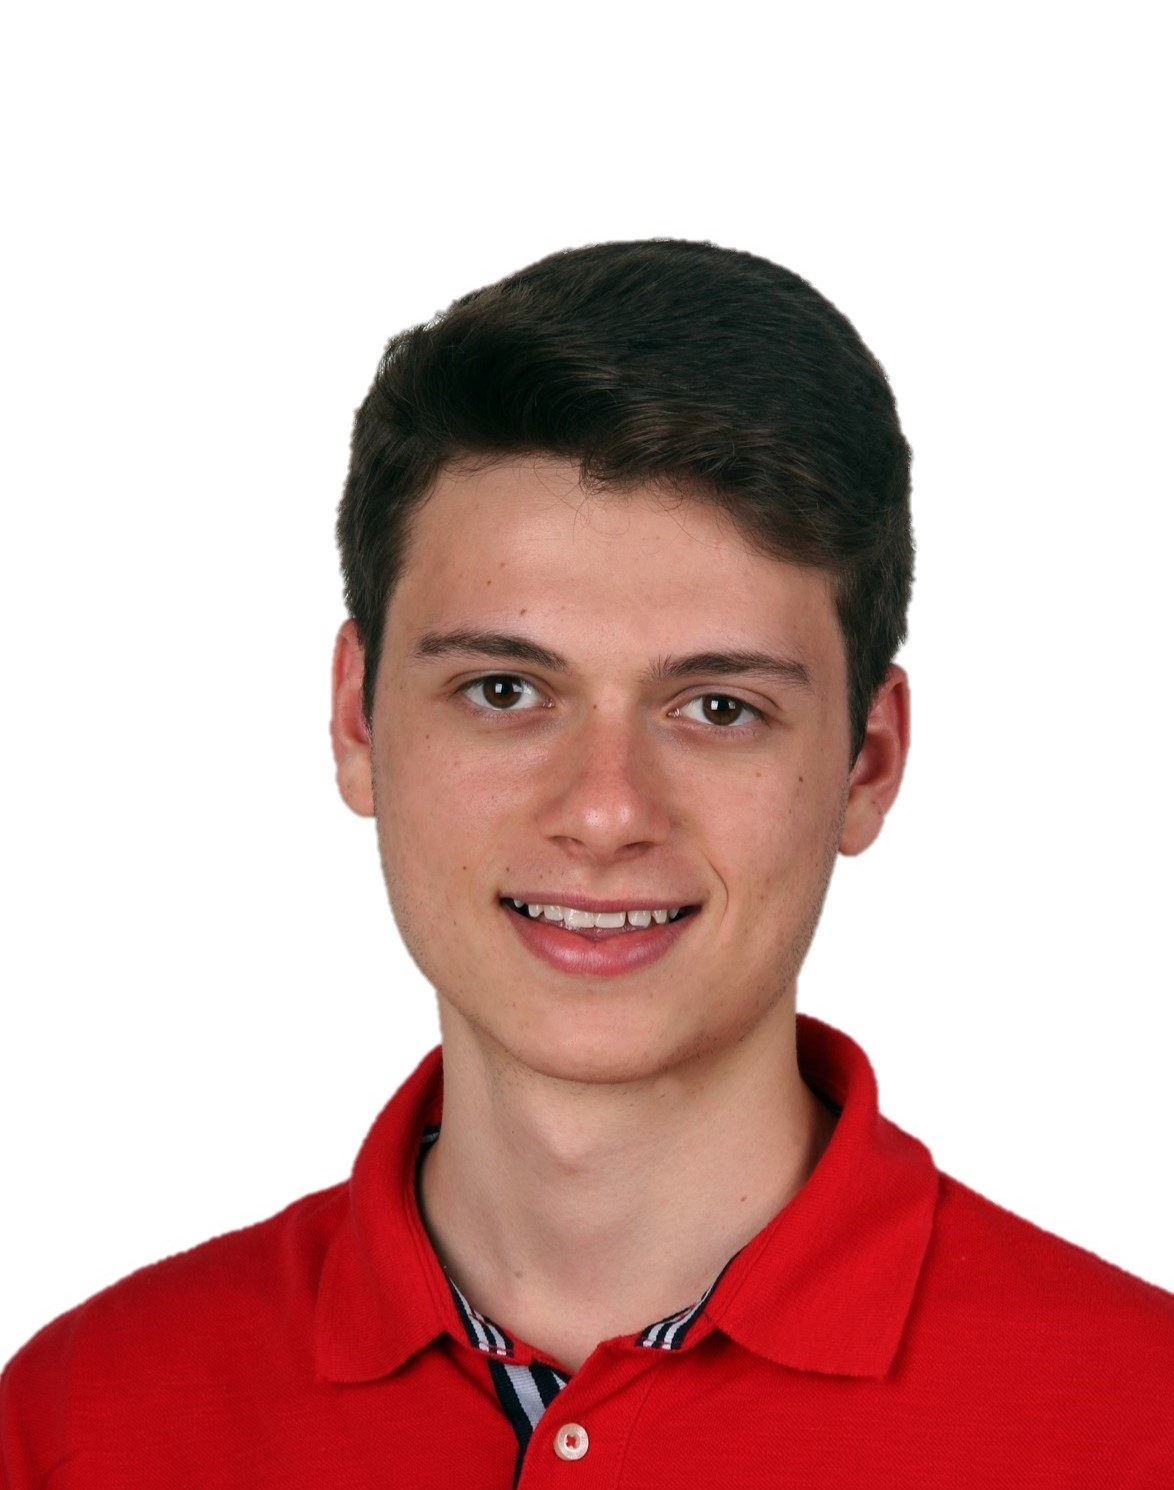
\includegraphics[scale=0.4]{Images/profile}};
\end{tikzpicture}
%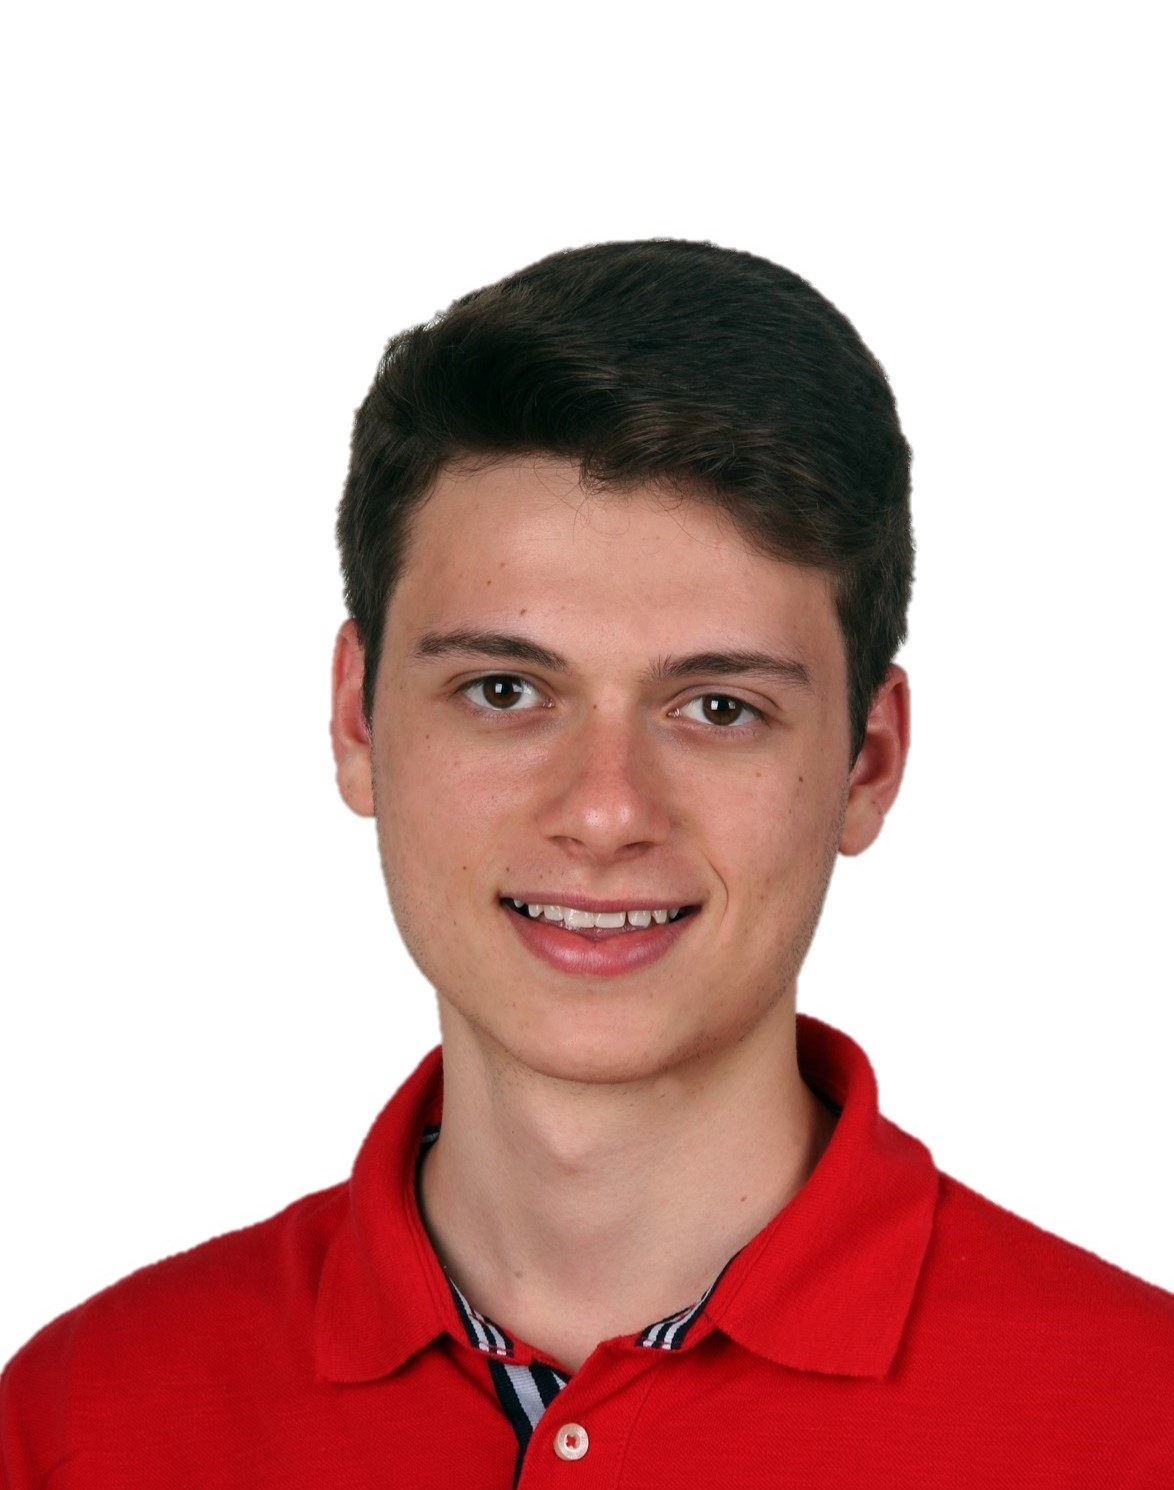
\includegraphics[scale=0.4]{Images/profile}  % uncomment for non-circular frame (and comment the 3 lines above)
\end{minipage}
\begin{minipage}{10.5cm}
\vspace{-1em}
\centerline{\Huge \textbf{Hugo Pereira}}
\vspace{8pt}
\centerline{\large \href{mailto:hugo.c.pereira@tecnico.ulisboa.pt}{hugo.c.pereira@tecnico.ulisboa.pt}}
\centerline{\large (+351) 96 33 62 767}
\centerline{\large Lisbon, Portugal} 
\vspace{8pt}
%\centerline{\href{https://www.linkedin.com/in/hugoacpereira/}{
\includegraphics[height=10pt]{Images/linkedin}~\footnotesize{linkedin.com/in/hugoacpereira/}}}
\href{https://www.linkedin.com/in/hugoacpereira/}{
\includegraphics[height=10pt]{Images/linkedin}~\footnotesize{linkedin.com/in/hugoacpereira/}}
\quad
\href{https://github.com/hugopereira-eng}{
\includegraphics[height=10pt]{Images/github}~\footnotesize{github.com/hugopereira-eng}} 
\end{minipage} 
\vspace{-10pt}



%-------------------------------SUMMARY--------------------------------
%\section{Summary}
%
%I am an early stage researcher in the Institute for Systems and Robotics (ISR) at Instituto Superior Técnico, University of Lisbon (IST/UL), interested in understanding robot motion under challenging nonlinear dynamics. I obtained my M.Sc. and B.Sc. degrees in Aerospace Engineering from IST/UL in 2022 and 2020, respectively. During this period, I was part of a one-year exchange program at the Technical University of Denmark (DTU). Throughout my academic career, I have been actively engaged in multiple student projects, including being part of the team that set the world record for the highest apogee ever achieved by a bi-liquid rocket built by university students, achieved during the European Rocketry Challenge (EuRoC), in 2021. One year later, in 2022, I participated in the largest Formula Student event globally, the Formula Student Germany competition, with the FST Lisbon team, achieving an impressive third place in the driverless cup. Some weeks later, the team went on to secure first place in the driverless category at the Formula Student Spain competition. During my academic years, I was distinguished with two Merit Awards endowed by IST/UL, and one Outstanding Performance at EuRoC 2021 Award endowed by DTU.  Some of my research areas include nonlinear control, dynamical systems, optimization theory, and reinforcement learning, with applications in space robotics.
 
 

%------------------------------EDUCATION-------------------------------
\section{Education}

\Education{Instituto Superior Técnico, University of Lisbon}{Aug.~2020 - Nov.~2022}{Master of Science in Aerospace Engineering~~(Control \& Systems branch)}{GPA:~19~/~20}

\vspace{5pt}
 
\Education{Technical University of Denmark}{Aug. 2020 - June 2021}{Exchange Student }{GPA:~11~/~12}

\vspace{5pt}

\Education{Instituto Superior Técnico, University of Lisbon}{Sep. 2017 - July 2020}{Bachelor of Science in Aerospace Engineering}{GPA:~17~/~20}

\vspace{5pt}

\Education{European Space Agency}{Mar. 2022}{Ladybird Guide to Spacecraft Communications Training Course}{}

\vspace{5pt}

\Education{University of Twente}{Aug. 2019}{Summer course in Robotics}{}



%-----------------------------EXPERIENCE-------------------------------
\section{Experience}

\Company{Institute for Systems and Robotics $\vert$ ISR Lisbon}{}
\Position{Fellow Researcher}{Jan. 2023 - Present}
\ItemListStart
        \ItemWithoutTitle{Currently doing research on spacecraft attitude control, using knowledge from optimal control, numerical optimization, attitude dynamics, and reinforcement learning.} \\
\ItemListEnd
\Position{Student Researcher}{Mar. 2022 - Dec. 2022}
\ItemListStart
        \ItemWithoutTitle{Worked towards my master's thesis titled \textit{"A Convex Allocation Framework for Singularity Avoidance in Control Moment Gyro Clusters"}, which was awarded the grade of 20 out of 20.}
        \ItemWithoutTitle{Developed algorithms for precise spacecraft maneuvering in the presence of singularities. The proposed solutions involved control theory, convex optimization, and advanced algebra concepts.}
\ItemListEnd 

\Company{Formula Student Lisbon $\vert$ FST Lisbon}{}
\Position{Autonomous Systems Engineer}{Sep. 2021 - Sep. 2022}
\ItemListStart
        \ItemWithoutTitle{Developed autonomous driving algorithms, using ROS/C++, for a driverless Formula car. The algorithms derived encompassed machine learning for point-cloud processing, state estimation via Kalman filter, simultaneous localization and mapping (SLAM), and model predictive control (MPC).}
        \ItemWithoutTitle{Competitions: Formula Student Germany 2022, $3^{rd}$ place in the Driverless Cup; Formula Student Spain 2022, $1^{st}$ place in the Driverless Cup.}
\ItemListEnd

\Company{Danish Student Association for Rocketry $\vert$ DanSTAR}{}
\Position{Avionics Systems Engineer}{Nov. 2020 - Oct. 2021}
\ItemListStart
        \ItemWithoutTitle{Member of the electronics department that was in charge of the development of the electrical systems of the rocket. I designed and tested multiple PCBs of the flight computer and was responsible for the telemetry and tracking system. In the end, I carried out flight trajectory simulations, using the OpenRocket software, that resulted in a predicted apoogee error of less than 3\%.}
         \ItemWithoutTitle{Competition: European Rocketry Challenge 2021, Portugal; Received the 9km flight category award; The team set the altitude world record for collegiate bi-liquid rocketry with an apogee of 6545m AGL.}
\ItemListEnd

\Company{Aerospace Engineering Students Group $\vert$ AeroTéc}
{}
\Position{Student Member}{Oct. 2018 -  June 2020}
\ItemListStart
        \ItemWithoutTitle{Part of the UAV-ART project, whose goal was to design an autonomous fixed-wing aircraft to navigate through predefined waypoints. During my first year, I was involved in the design and construction of the UAV. In my second year, I took part in the development of the flight controller, which involved PID control, filtering, path planning, sensor fusion, and system identification algorithms. The simulations were carried out in \textsc{Matlab}/\textsc{Simulink} and the on-board controller was implemented in an RPi.}%Tech used: MATLAB/Simulink, Raspberry Pi.
        \ItemWithoutTitle{Gave workshops about rocketry to high schools and college students. These consisted of a hands-on experience in planning, building and launching a small rocket made of cheap conventional materials.} %In total, I gave six sessions.
\ItemListEnd

\Company{UAVision}{}
\Position{Summer Intern}{June 2021 - July 2021}
\ItemListStart
        \ItemWithoutTitle{Short-term internship where I worked on the development of a signal demodulation program for an Emergency Position Indicating Radio Beacon system. The program was written in Python, in collaboration with other interns.}
\ItemListEnd



%----------------------------------SKILLS------------------------------------
\section{Skills Summary}

\vspace{-10pt}

\begin{align*}
&\text{\textbf{Languages}} &&\text{English (C1 certificate), Portuguese (Native)}\\
&\text{\textbf{Programming}} &&\text{C++, C, \textsc{Matlab}, Python} \\
&\text{\textbf{Software}} &&\text{\textsc{Simulink}, KiCad, OpenRocket, SolidWorks}\\
&\text{\textbf{Tools}} &&\text{Git, \textsc{LaTex}, Microsoft Office}\\
&\text{\textbf{Platforms}} &&\text{Linux, Windows, ROS, STM32, PIC24, Arduino}\\
&\text{\textbf{Miscellaneous}} &&\text{Soldering, Driving License}
\end{align*}



%--------------------------VOLUNTEERING-----------------------------
\section{Volunteering}

\Company{Erasmus Student Network, DTU section}{Feb. 2021 - June 2021}
\ItemListStart
        \ItemWithoutTitle{Member of a multinational team of volunteers whose goal is to facilitate the integration of international students in the local community.}
        \ItemWithoutTitle{Organized social events and provided general support and guidance for exchange students.}
\ItemListEnd



%-------------------------------AWARDS----------------------------------
\section{Honours and Awards}

\begin{description}[font=$\circ$]
\itemsep-2pt 
\item {Outstanding Performance at EuRoc 2021, DTU Blue Dot, Oct. 2021}
\item {Academic Merit, Instituto Superior Técnico, 2017/2018, 2019/2020}
\item {Best Student Award, Escola Secundária Marquesa de Alorna, 2015/2016, 2016/2017}
\end{description}



%----------------------------CERTIFICATES-----------------------------
%\section{Certificates}
%
%\begin{description}[font=$\circ$]
%\itemsep-2pt 
%\item {Online Ladybird Guide to Spacecraft Communications Training Course, 2022, ESA Academy}
%\item {Drone Simulation and Control, 2020, MOOC TÉCNICO}
%\item {European BEST Engineering Competition, 2018, BEST}
%\end{description}



%----------------------------ACTIVITIES---------------------------------
\section{Hobbies and Activities}

\begin{description}[font=$\circ$]
\itemsep-2pt
\item {Running, swimming, travelling, and playing the guitar.}
\item {Practiced athletics as a federated athlete for 8 years (2009-2017) while competing at the national level.}
\end{description}



\end{document}